% !TEX TS-program = xelatex
% !TEX encoding = UTF-8 Unicode
% -*- coding: UTF-8; -*-
% vim: set fenc=utf-8

%%%%%%%%%%%%%%%%%%%%%%%%%%%%%%%%%%%%%%%%%%%%%%%%%%%%%%%%%%%%%%%%%
%% CV.tex
%% <https://github.com/zachscrivena/simple-resume-cv>
%% This is free and unencumbered software released into the
%% public domain; see <http://unlicense.org> for details.
%%%%%%%%%%%%%%%%%%%%%%%%%%%%%%%%%%%%%%%%%%%%%%%%%%%%%%%%%%%%%%%%%

% See "README.md" for instructions on compiling this document.

\documentclass[letterpaper,MMMyyyy,nonstopmode]{simpleresumecv}
% Class options:
% a4paper, letterpaper, nonstopmode, draftmode
% MMMyyyy, ddMMMyyyy, MMMMyyyy, ddMMMMyyyy, yyyyMMdd, yyyyMM, yyyy

%%%%%%%%%%%%%%%%%%%%%%%%%%%%%%%%%%%%%%%%%%%%%%%%%%%%%%%%%%%%%%%%%
%% PREAMBLE.
%%%%%%%%%%%%%%%%%%%%%%%%%%%%%%%%%%%%%%%%%%%%%%%%%%%%%%%%%%%%%%%%%

% CV Info (to be customized).
\newcommand{\CVAuthor}{ Yasaman Mirmohammad}
\newcommand{\CVTitle}{Yasaman's CV for Acme Corporation}
\newcommand{\CVNote}{CV compiled on {\today} for Acme Corporation}
\newcommand{\CVWebpage}{}

% PDF settings and properties.
\hypersetup{
pdftitle={\CVTitle},
pdfauthor={\CVAuthor},
pdfsubject={\CVWebpage},
pdfcreator={XeLaTeX},
pdfproducer={},
pdfkeywords={},
unicode=true,
bookmarks=true,
bookmarksopen=true,
pdfstartview=FitH,
pdfpagelayout=OneColumn,
pdfpagemode=UseOutlines,
hidelinks,
breaklinks}

% Shorthand.
\newcommand{\Code}[1]{\mbox{\textbf{#1}}}
\newcommand{\CodeCommand}[1]{\mbox{\textbf{\textbackslash{#1}}}}

%%%%%%%%%%%%%%%%%%%%%%%%%%%%%%%%%%%%%%%%%%%%%%%%%%%%%%%%%%%%%%%%%
%% ACTUAL DOCUMENT.
%%%%%%%%%%%%%%%%%%%%%%%%%%%%%%%%%%%%%%%%%%%%%%%%%%%%%%%%%%%%%%%%%
\usepackage{graphicx}
\graphicspath{ {./image/} }

\begin{document}

%%%%%%%%%%%%%%%
% TITLE BLOCK %
%%%%%%%%%%%%%%%

\Title{\CVAuthor}

\begin{SubTitle}
\href{https://www.google.com/maps/place/Amirkabir+University+of+Technology+(Polytechnic}
{Department of Computer Engineering and Information Technology, Amirkabir University of Technology, 424 Hafez Ave., Tehran, Iran}
\par
\,\SubBulletSymbol\,
\href{yasaman.m.1997@gmail.com}
{yasaman.m.1997@gmail.com}

\href{ys.m@aut.ac.ir}
\,\SubBulletSymbol\,
{ys.m@aut.ac.ir}

\,\SubBulletSymbol\,
+98\,9120630714

\href{https://www.linkedin.com/in/yasaman1997/}
\,\SubBulletSymbol\,
{https://www.linkedin.com/in/yasaman1997/}

\href{\CVWebpage}
{\url{\CVWebpage}}
\end{SubTitle}

%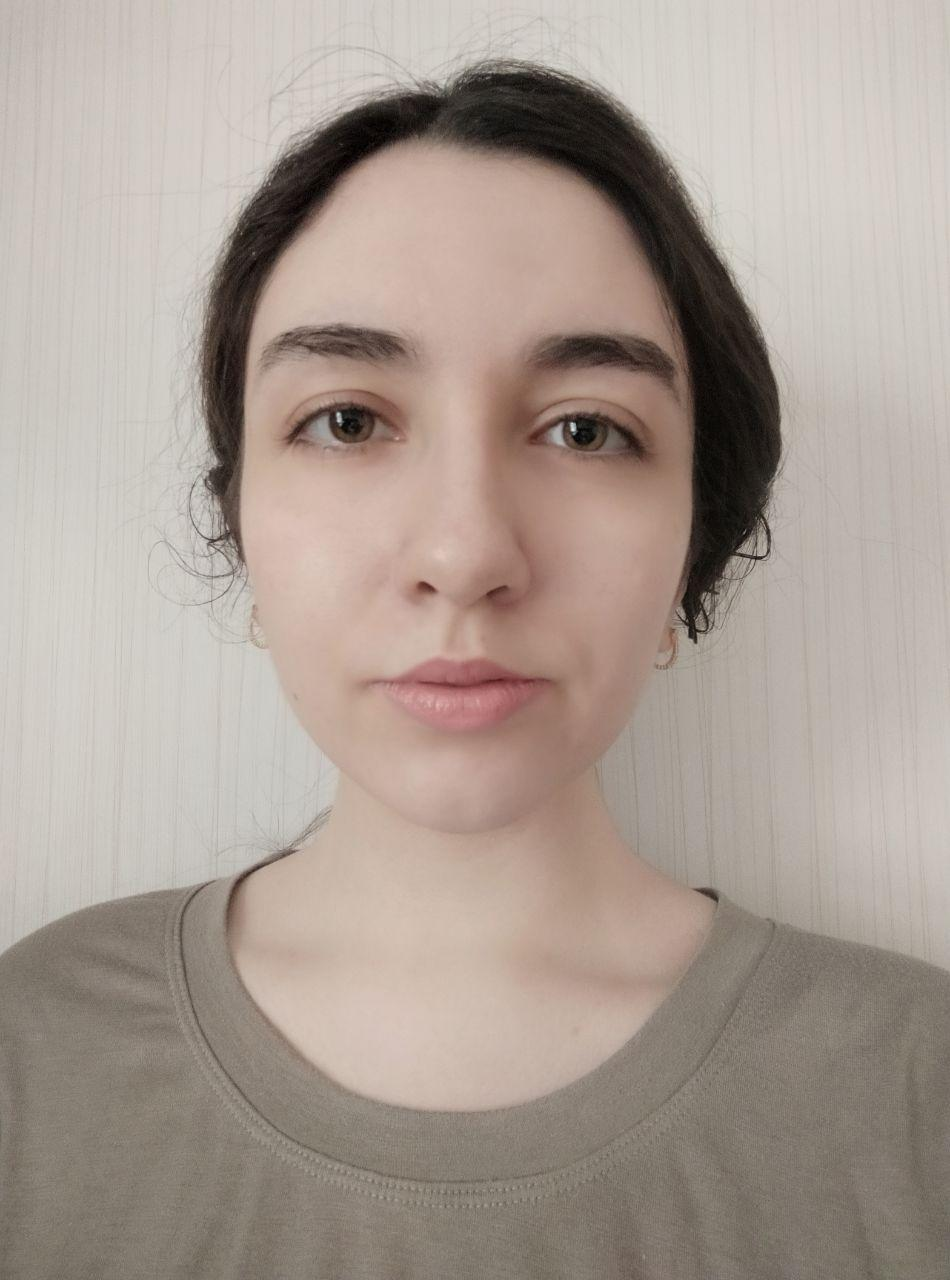
\includegraphics[scale=0.2]{image/2.jpg}

\begin{Body}

%%%%%%%%%%%%%%%
%% EDUCATION %%
%%%%%%%%%%%%%%%
\Section
{RESEARCH INTERESTS}
{RESEARCH INTERESTS}
{PDF:Interests}

\Entry

\BulletItem
Machine Learning
\BulletItem
Bioinformatics
\BulletItem
Computer Vision
\BulletItem
Cognitive science




\Section
{Education}
{Education}
{PDF:Education}

\Entry
\href{http://www.aut.ac.ir}
{\textbf{Amirkabir University of Technology}},
Tehran, Iran

\Gap
\BulletItem
B.S. in
\href{http://ceit.aut.ac.ir}
{Computer Engineering}, 
 \BulletItem
 \textbf {GPA(selected courses): 16.6/ 20} ,including:
 
Mathematics2
Engineering Statistics,
Logic design,
Logic Circuits & Computer Architecture Laboratory,
Technical English,
Research & Technical Presentation,
Digital Electronics,
Operating Sys. Design (I),
Electronic Circuits Lab,
Microprocessor (I) and Assembly Language,
Microprocessors (I) Lab,
Computer Architecture Internship,
Foundations of Data Mining,
Engineering Economics,
Signals and Systems,
Database Design Lab,
Digital Electronics Lab,
Special Topics (Information Security),
Programmable Digital Systems Design,
Discrete Mathematics,
English for the Students of Engineering

\Gap
\newline

\BulletItem
  \textbf {GPA(last 4 semester): 15.25/20,Passed Credits: 56}
 
 \BulletItem
 \textbf {GPA(Total): 14.16/20,Passed Credits: 121}
\hfill
\DatestampYM{2015}{09} -- \DatestampYM{2019}{09} 
\href{}
\Entry
{\textbf{Sama School(2008-2014) , Sadra School(2014-2015)}},
Tehran, Iran
\BulletItem
Diploma in Mathematics and Physics Discipline, 
GPA: 19.78/20
\hfill
\DatestampY{2010}--
\DatestampY{2015}

\begin{Detail}

\end{Detail}


\BullENCE %%
%%%%%%%%%%%%%%%%%%%%%%%%%

\Section
{Research Experience}
{Research Experience}
{PDF:ResearchExperience}

\Entry
\href{}
\BulletItem
{\textbf{IPM,School of Cognitive sciences}} 
\newline (Researcher,under supervision of \href{https://scholar.google.de/citations?user=H3AwrOAAAAAJ&hl=en}{Dr Moein Esghaei})
\hfill
\DatestampYM{2019}{05} --
Now
\begin{Detail}
\SubBulletItem
This project is in cooperation between the IPM School of cognitive sciences, UCLA’s Brain research institute, and the German Primate Center. The project focuses on the physiological origins of attention in the monkey brain.  
\end{Detail}


\Entry
\href{}
\BulletItem
{\textbf{Bio-Inspired System Design Lab}} 
\newline (Amirkabir University of Technology,Iran,Tehran)
\hfill
\DatestampYM{2018}{05} --
\DatestampYM{2019}{9}
\begin{Detail}
\SubBulletItem
Design and Implementation of a knn-regression based method for ball trajectory prediction 
\end{Detail}


\Entry
\href{}
\BulletItem
{\textbf{Shahid Rajaee Teacher Training University,
Iran,Tehran}}
\hfill
\DatestampYM{2018}{08} --
\DatestampYM{2019}{11}

\begin{Detail}
\SubBulletItem
Implementation of a congnitive style based English Learning Application 
\end{Detail}


\BulletItem
{\textbf{Lab of Brain and Cognitive science}} 
\newline (Royan Institute of Research,Iran,Tehran)
\hfill
\DatestampYM{2018}{01} --
\DatestampYM{2019}{1}
\begin{Detail}
\SubBulletItem
Internship under Supervision of Dr.M.Khaligh Razavi
\end{Detail}
\begin{Detail}
\SubBulletItem
Disease Trajectory Detection via Deep learning,under Supervision of
\href{https://scholar.google.co.uk/citations?user=3HbeiywAAAAJ&hl=en}{Dr Mahdi Khaligh Razavi}
\end{Detail}



\BulletItem
{\textbf{Big Data Lab}} 
\newline (Amirkabir University of Technology,Iran,Tehran)
\hfill
\DatestampYM{2018}{06} --
\DatestampYM {2018}{10}
\begin{Detail}
\SubBulletItem
DeepFM: A Factorization-Machine based Neural Network for CTR Prediction
\SubBulletItem Wide and Deep Graph Convolutional Neural Network Matrix Completion
\newline under Supervision of Dr.M.Amihaeri 
\end{Detail}



\Entry
\href{}
\BulletItem
{\textbf{Lab Of Robotics and Cognitive science}} 
\newline (Amirkabir University of Technology,
Iran,Tehran)
\hfill
\DatestampYM{2017}{08} --
\DatestampYM{2017}{12}


\begin{Detail}
\SubBulletItem
Project: Datamining and Cognitive science concepts

\end{Detail}






%\SubBulletItem
%Supervisors:

%\SubBulletItem
%Focus:




\Gap

%%%%%%%%%%%%%%%%%%
%% PUBLICATIONS %%
%%%%%%%%%%%%%%%%%%
%%%%%%


%%%%%%%%%%%%%%%%%%%%%%%%%%%
%% AWARDS & SCHOLARSHIPS %%
%%%%%%%%%%%%%%%%%%%%%%%%%%%

\Section
{Honors \&\newline
Awards}
{Honors \& Awards}
{PDF:HonorsANDAwards}


\BulletItem
  Awarded fellowship,undergraduate program,Department of Computer Engineering, Amirkabir University of Technology
  \hfill
\DatestampYM{2015}{09} --
Now


\BulletItem
  Member of Coursera Mentoring Team(IBM Courses):
  \hfill
\DatestampYM{2018}{08} --
Now
   \begin{itemize}
       \item Fundamentals of Scalable Data Science
         \item  Advanced Machine Learning and Signal Processing
           \item Applied AI with DeepLearning  
             \item    Advanced Data Science Capstone
   \end{itemize}
\hfill


\BulletItem
Ranked top 0.4 \% among more than 180,000 students participated
in the\newline nationwide entrance examination of undergraduate studies
in Iranian universities  
\hfill
\DatestampY{2014} --
\DatestampY{2015}

\BulletItem
 accepted for 2nd level of computer Olympiad 
\hfill
\DatestampYMD{2013}


\BulletItem
 Member of National Organization for Bilingual Schools
\hfill
\DatestampYMD{2007} --
\DatestampYMD{2014}


\Section
{Publications}
{Publications}
{PDF:Publications}
\begin{itemize}
    
\item
{[1] Wide and Deep Graph Convolutional Neural Network Matrix Completion, (To Be Submitted)
\hfill
%\DatestampYMD{2018} --

}

\item
{[2] Ball Path prediction for humanoids:Combination of KNN regression and Autoregression methods, Yasaman Mirmohammad, Shayan Khorsandi, Mohammad Navid Shahsavari, Behnam Yazdankhoo, Soroush Sadeghnejad,accepted to the ICRoM conference 2019, Jul 2019}
\end{itemize}

%%%%%%%%%%%%%%%%%%%%%%%%%%%%%%%%%%%%%%%%%%%%
%% Conference %%
%%%%%%%%%%%%%%%%%%%%%%%%%%%%%%%%%%%%%%%%%%%%
\Section
{Conferences}
{Conference}
{PDF:Conferences}

\Entry
\textbf{Colombia BME Webinar}
\hfill
Fall \DatestampYM{2020-2021}

\BulletItem
Instructor: Biomedical Engineering Department,Colombia University 

\Entry
\textbf{IPM Cognitive Neuroscience Journal Clubs}
\BulletItem
Instructor: Dr. Moein Esghaei
\hfill
\DatestampYM{2019-2020}

\Entry
\textbf{Royan Summer school,on Fundamentals of Cognitive Science}
\BulletItem
Instructor: Dr. Seyed Mehdi Khaligh Razavi
\hfill
Summer\DatestampYM{2018}


%%%%%%%%%%%%%%%%%%%%%%%%%%%%%%%%%%%%%%%%%%%%
%% PROFESSIONAL AFFILIATIONS & ACTIVITIES %%
%%%%%%%%%%%%%%%%%%%%%%%%%%%%%%%%%%%%%%%%%%%%

\Section
{Teaching Experience}
{Teaching Experience}
{PDF:ResearchExperience}

\Entry
\textbf{Principles of Datamining},Amirkabir University of Technology
\hfill
Fall \DatestampYM{2019}

\BulletItem
Instructor: Dr. Khabbaz

\Entry
\textbf{Principles of Datamining},Amirkabir University of Technology
\hfill
Spring \DatestampYM{2019}

\BulletItem
Instructor: Dr.E.Nazerfard

\Entry
\textbf{Principles of Programming},Amirkabir University of Technology
\hfill
Fall\DatestampYM{2018}

\BulletItem
Instructor: Dr.E.Nazerfard

\Entry
\textbf{Probability and statistics},Amirkabir University of Technology
\hfill
Fall\DatestampYM{2018}

\BulletItem
Instructor: Dr M.Amirhaeri

\Entry
\textbf{Digital Electronic},Amirkabir University of Technology
\hfill
Fall\DatestampYM{2018}

\BulletItem
Instructor: Dr H.Farbeh


\Entry
\textbf{Discrete Mathematics},Amirkabir University of Technology
\hfill
Spring \DatestampYM{2016}

\BulletItem
Instructor: Dr.m.s.Fallah


\Entry
\textbf{Discrete Mathematics,Algebra and Geometry},Sadra School
\hfill
Fall \DatestampYM{2016}

\BulletItem
Instructor: Dr.m.Rashedi



\Entry
\textbf{Fundamentals of Physics},Sadra School
\hfill
Fall \DatestampYM{2016}

\BulletItem
Instructor: A.Jamshidi



% Manual page break.

%%%%%%%%%%%%%%%%%%%%%%%
%% CAMPUS ACTIVITIES %%
%%%%%%%%%%%%%%%%%%%%%%%


%%%%%%%%%%%%%%%%%%%%%%%%%%%
%% OTHER WORK EXPERIENCE %%
%%%%%%%%%%%%%%%%%%%%%%%%%%%


%%%%%%%%%%%%%%%
%% LANGUAGES %%
%%%%%%%%%%%%%%%

\Section
{Language Skills}
{Language Skills}
{PDF:Languages}

\BulletItem
\textbf{Persian}: Native language.

\Gap
\BulletItem
\textbf {English}: Fluent (speaking, reading, writing).

\Gap
\BulletItem
\textbf{French}: Basic (reading); basic (speaking, writing).

%%%%%%%%%%%%
%% SKILLS %%
%%%%%%%%%%%%

\Section
{Technical Skills}
{Skills}
{PDF:Skills}

\Entry

\begin{itemize}
\item \textbf {Programming and Development}
\begin{itemize}
    \item Python(2,3)
    \item C,C++
    \item Java
    \item MATLAB
    \item HTML+CSS
    \item JavaScript
    \item php
    
\end{itemize}



    \item \textbf{ Software libraries and distributions}: 
    \begin{itemize}
        \item OpenCV
        \item Tensorflow
        \item Keras
        \item Yolo
        \item Cuda and Openmp
        \item NLTK and Gensim
    \end{itemize}
     


\item \textbf {DataBase Design}
\begin{itemize}
     \item MySQL
     \item NoSQL(MongoDB)

\end{itemize}


 \item \textbf{Others}: 
\item{\LaTeX}
\item Microsoft Word,Excel,PowerPoint

\end{itemize}






%%%%%%%%%%%%%%%%
%% Projects %%
%%%%%%%%%%%%%%%%

\Section
{Projects}
{Projects}
{PDF:Projects}

\Entry
\begin{itemize}
	\item \textbf{Data Structure} :
		\begin{itemize}
		\item	search engine using inverted index algorithm(C++)
	     \item   Finite-State Automata (Java)
		\end{itemize}
		
	\item \textbf{Advanced Computer Programming}:
		\begin{itemize}
		\item  Implementation of a graphical game (BattleShip-Online) (Java)
     	\item Implementation of a simple image editor (Java)
	    \item Implementation of a simple Encryption and encoding System  (Java)
		\end{itemize}
		
	\item \textbf{Principles of Computer and Programming }: 
		\begin{itemize}
	    \item  living cell simulation (C)
	      	\end{itemize}
   	\item \textbf{Logic Design} : 
   		\begin{itemize}
     \item	Designing a Traffic Light System (Verilog)
     		\end{itemize}
   	\item \textbf{Computer Architecture and design} :
   		\begin{itemize}
		\item Basic Computer,Compiler,Cache,Pipeline(VHDL)
		\end{itemize}
		
     \item \textbf{Operating Systems}:
     \begin{itemize}
       \itemMultiprocessing,Multithreading in Windows and Linux(C)
		\end{itemize}
	

	
	\item \textbf{Design Automation}:
		\begin{itemize}
		\item Phase1:Implementation of a car parking system(VHDL).
     	\item Phase2:Implementation of a co-software,hardware design using
     	      Microblaze(VHDL).
	    \item Phase3:Implementation of a Plant-Watering System with a moisturizing
	          detection system(VHDL)
	          
		\end{itemize}
		
			\begin{itemize}
		\item Implementation of a word-detector system using  "LSTM" Neural Networks, designing and Implementation on FPGA.
	          
		\end{itemize}
		
	
		
    \item \textbf{Advanced Mathematics}: 
	    \begin{itemize}
        \item Phase1:Analyzing Distribution categories of a two class  problem And PCA(Python,MATLAB)
		      \item Phase2:
     	     Facial Recognition with Singular Value Decomposition(Python)
     	     based on 	\href{https://link.springer.com/chapter/10.1007/978-1-4020-6264-3_26}{paper}
     \end{itemize}
      
   
       	  \item \textbf{Artificial Intelligence}: 
	    \begin{itemize}
        \item 
		  Implementation of Classical and Non-Classical searches(BFS,DFS,Simulated annealing,Hill Climbing,Genetic) - (Python,Java,C++)
     \end{itemize}
     
     
       	  \item \textbf{Principles of Data Mining}: 
	    \begin{itemize}
        \item 
	Basic Methods and Algorithms of Supervised and Unsupervised Learning, all available \href{https://github.com/Yasaman1997/DataMining_and_DataAnalysis/tree/master/DM_2018/HWS}{here}(Python)
     \end{itemize}
     
\item \textbf{Principles Web programming}: 
	    \begin{itemize}
        \item 
Front-end & Back-end programming.
project was based on deigning \href{https://www.reyhoon.com/} {\textbf{Reyhoon}} website. you can find it here:\href{https://github.com/Yasaman1997/Internet_Engineering}{here}
     \end{itemize}
     

  
  
  
     
  \end{itemize}	
 	


%%%%%%%%%%%%%%%%
%% Challenges And Self Studies %%
%%%%%%%%%%%%%%%%

\Section
{Challenges And Self Studies}
{Challenges And Self Studies}
{PDF:Challenges And Self Studies}

\Entry
\begin{itemize}
    \item \textbf{Contests}

\begin{itemize}

\item \textbf {Amirkabir First Data mining Challenge}(Fall 2017)
    	
   \begin{itemize}
	   
     \item Analyzing the bank customer's  information
     \item Predicting the result
   
    \end{itemize}
	
		

\item \textbf {Deca Dataminig challenge}, Sharif University of Technology(Winter2018)
 \begin{itemize}
	   
     \item Analyzing the Notification of an App and the effect of different kind of notifs on the satisfaction of the users.
    
   
    \end{itemize}
	
	
\item \textbf {Fanavard Dataminig challenge},(Spring 2018)
 \begin{itemize}
	   
     \item Analyzing and predicting of gold cost considering the cost in previous months
     \item Ranked top 7 teams for the final level(Summer 2018)
    
   
    \end{itemize}



\item \textbf {Amirkabir 2nd Data mining Challenge}(Winter 2019)
    	
   \begin{itemize}
	   
     \item Time Series Analysis with LSTMc and Arima models
  
   \end{itemize}


\item     \textbf{ Sharif Machine Learning Workshop}(Winter 2018):
	      \begin{itemize}
	          \item Python Libraries for machine learning,Deep learning:Keras, Tensorflow
	      
	      
	      \end{itemize}

         	\item 
      \href{ https://www.kaggle.com/c/dog-breed-identification}{"Dog Breed Identification Challenge "} (Kaggle,Winter 2018)
      

 
        	\item 
      \href{https://www.kaggle.com/c/tensorflow-speech-recognition-challenge}{"TensorFlow Speech Recognition Challenge "} (Kaggle,Spring 2018)
 
   \end{itemize}     
       \end{itemize}  
        
 \begin{itemize}
    \item \textbf{Courses}
    \begin{itemize}
    
     \item \href {https://coursera.org/share/ef186768574d9675b6eeedfc9afab371}{Mathematics for Machine Learning Specialization: Linear Algebra,pca and calculus}(September 2018)
           
    \item \href {https://coursera.org/share/1bde1eaf453c5df48f61d5d53ce4ee0c}{Deep Learning Specialization, from Deeplearning.ai}(June 2020)
           

      \item \href {https://coursera.org/share/2e19ff0d0105de605193e29661a7458d}{Big data Specialization, University of California San Diego}(March 2020)

      \item \href {https://coursera.org/share/2e19ff0d0105de605193e29661a7458d}{AI for medicine Specialization, from Deeplearning.ai}(May 2020)
        
        
         \item  \href {https://www.coursera.org/learn/machine-learning}{Machine Learning, by Stanford University on Coursera}
       	  
        \item \href {https://www.coursera.org/learn/neural-networks}{Neural Networks for Machine Learning, by University of Toronto on Coursera}
        

         \item \href{https://www.coursera.org/learn/intro-to-deep-learning}{Introduction to Deep Learning, by National Research University Higher School of Economics on Coursera}
         
       \item \href{https://www.coursera.org/account/accomplishments/certificate/3QC9VVKDHVYD}{Natural Language Processing,by National Research University Higher School of Economics on Coursera}
       
       \item\href{https://www.coursera.org/account/accomplishments/certificate/RGJ87CLXQTNV}{Introduction to Research for Essay Writing}
       
       \item \href{https://www.coursera.org/account/accomplishments/certificate/35UZFCGDFMM5}{Basic Statistics}
       \item \href{https://www.coursera.org/account/accomplishments/certificate/VB32F5YFWLY5}{How to Win a Data Science Competition: Learn from Top Kagglers (with Honors)}
       \item \href{https://www.coursera.org/account/accomplishments/certificate/A4XCM3ZN73ES}{Practical Machine Learning}
       \item \href{https://www.coursera.org/account/accomplishments/certificate/7VVUS8ZEKXCK}{Advanced Writing}
       \item \href{https://www.coursera.org/account/accomplishments/certificate/W2VSLW8B6VSF}{Fundamentals of Scalable Data Science}
       \item \href{https://www.coursera.org/account/accomplishments/certificate/VFYNXNR8UEMR}{Graph Analytics for Big Data}
    
    
            
            \item \href {https://www.coursera.org/account/accomplishments/certificate/2L2LR5CLCKV3}
            {Fashion as Design,The Museum of Modern Art}
        
         
                 \item \href {https://www.coursera.org/account/accomplishments/verify/SHNVDERAXLHU}{Introduction to Data Science in Python}(September 2018)
             
        
        \item \href {https://www.coursera.org/account/accomplishments/certificate/RPZJQLVQJAC3}{English for Career Development}(May 2020)
        
        \item \href {https://www.coursera.org/account/accomplishments/certificate/DSDTJAJ225PF}{Machine Learning With Big Data}(May 2020)
        
        \item \href {https://www.coursera.org/account/accomplishments/certificate/N4B2R35GAXB2}{    Databases and SQL for Data Science}(May 2020)
        
        
        \item \href {https://www.coursera.org/account/accomplishments/certificate/7H53FKHFAEGQ}{Data Science Math Skills}(May 2020)
        
        
        \item \href {https://www.coursera.org/account/accomplishments/certificate/5MV7NYYEZ7SQ}{   Convolutional Neural Networks in TensorFlow}(May 2020)
        
       \item \href{https://www.coursera.org/account/accomplishments/certificate/LK22QA98NHP8}{    Introduction to Philosophy}
       \item \href{https://www.coursera.org/account/accomplishments/certificate/4MDAYTPAZDC2}{Philosophy of Science}
       \item \href{https://www.coursera.org/account/accomplishments/certificate/H65GN6U32DPY}{Biology Meets Programming: Bioinformatics for Beginners}
       \item \href{https://www.coursera.org/account/accomplishments/certificate/BUU9S5EZ9KK6}{Computational Neuroscience}
       \newline
        \item 
    Other courses and all certificates can be found \href{https://github.com/Yasaman1997/Certificates} {\textbf{Here}}
    \end{itemize}
  \end{itemize}
  
 \Section
{Lectures}
{Lectures}
{PDF:Lectures}

\Entry
\begin{itemize}
\item An introduction to computer security,Computer and IT department of Amirkabir University of Technology
  \hfill
\DatestampYM{2017}

\item Reinforcement Learning in Robotics, based on \href{https://ri.cmu.edu/pub_files/2013/7/Kober_IJRR_2013.pdf} {"Reinforcement Learning in Robotics:A Survey"};Computer and IT department of Amirkabir University of Technology
  \hfill
\DatestampYM{2018}

\item A LSTM based approach for disease trajectory, ;Royan institute,Cognitive Neuroscience lab,
  \hfill
\DatestampYM{2018-2019}

\item Sample presentation can be found  \href{https://github.com/Yasaman1997/Presentation/blob/master/bandicam%202020-08-01%2011-49-26-553.mp4} {\textbf{Here}}

\end{itemize}

%%%%%%%%%%%%%%%
%% INTERESTS %%
%%%%%%%%%%%%%%%

\Section
{Interests}
{Interests}
{PDF:Interests}

\Entry
Philosophy,
Painting ,
Badminton ,
Music ,  
Language  and communication ,
History,
Swimming
\Section
{References}
{References}
{PDF:References}

%%%%%%%%%%%%%%%%
%% REFERENCES %%
%%%%%%%%%%%%%%%%
\Entry
\begin{itemize}
\item seyed@cognetivity.com 
\item aesghaei@dpz.eu

\end{itemize}


\Section
{Further information}
{Further information}
{PDF:Further information}

\Entry
All Available in:\href{https://github.com/Yasaman1997} {\textbf{Github}}  





%%%%%%%%%%%%%%%%%%%%%%%%%%%%%%%%%%%
%% MULTILINGUAL UNICODE EXAMPLES %%
%%%%%%%%%%%%%%%%%%%%%%%%%%%%%%%%%%%









\end{Body}

%%%%%%%%%%%
% CV NOTE %
%%%%%%%%%%%


\end{document}
